%!TEX root=../../main.tex

\section{Exercises}

% Chapter 7 exercises
% 
% many problems drawn from OI 4 source files

%__________________
\subsection{Simple vs. multiple regression}

% 1 oi_biostat

\eoce{\qt{PREVEND, Part I\label{prevend_interpret}} The summary table below shows the results of a multiple regression model of RFFT score versus statin use and age. 

\begin{center}
\begin{tabular}{rrrrr}
	\hline
	& Estimate & Std. Error & t value & Pr($>$$|$t$|$) \\ 
	\hline
	(Intercept) & 137.8822 & 5.1221 & 26.92 & 0.0000 \\ 
	Statin & 0.8509 & 2.5957 & 0.33 & 0.7432 \\ 
	Age & -1.2710 & 0.0943 & -13.48 & 0.0000 \\
	\hline
\end{tabular}
\end{center}

In a clinical setting, the interpretive focus lies on reporting the nature of the association between the primary predictor and the response, while specifying which potential confounders have been adjusted for. Briefly respond to a clinician who is concerned about a possible association between statin use and decreased cognitive function, based on the above analysis.
}{}

% 2 oi_biostat

\eoce{\qt{PREVEND, Part II\label{prevend_causal}} Can the results of the analysis in Exercise~\ref{prevend_interpret} be used to conclude that as one ages, one's cognitive function (as measured by RFFT score) declines? Explain your answer.
}{}

% 3 ODD (OI4, 9.1 and 9.2) edited

\eoce{\qt{Baby weights, Part I\label{baby_weights_smoke_parity}} The Child Health 
and Development Studies investigate a range of topics. One study 
considered all pregnancies between 1960 and 1967 among women in the 
Kaiser Foundation Health Plan in the San Francisco East Bay area. The 
variable \texttt{smoke} is coded 1 if the mother is a smoker, and 0 if 
not. The variable \texttt{parity} is 1 if the child is the first born,
and 0 otherwise. The summary table below shows the results of a linear regression 
model for predicting the average birth weight of babies, measured in 
ounces, based on the smoking status of the mother and whether the child is the first born. 
\footfullcite{data:babies}

\begin{center}
\begin{tabular}{rrrrr}
  \hline
            & Estimate  & Std. Error  & t value   & Pr($>$$|$t$|$) \\ 
  \hline
(Intercept) & 123.57    & 0.72       & 172.75  & 0.0000 \\ 
smoke       & -8.96   & 1.03        & -8.68    & 0.0000 \\ 
parity & -1.98 & 1.15 & -1.72 & 0.0859 \\
  \hline
\end{tabular}
\end{center}

\begin{parts}
\item Write the equation of the regression model.
\item Interpret the model slopes in the context of the data.
\item Calculate the estimated difference in mean birth weight for two infants born to non-smoking mothers, if one is first born and the other is not. 
\item Calculate the estimated difference in mean birth weight for two infants born to mothers who are smokers, if one is first born and the other is not. 
\item Calculate the predicted mean birth weight for a first born baby born to a mother who is not a smoker.
\end{parts}
}{}

\textD{\newpage}

% 4 oi_biostat, from section 8, spring 2020

\eoce{\qt{Wolbachia, Part I\label{wolbachia_intro}} \textit{Wolbachia} is a microbial symbiont estimated to be hosted by about 40\% of all arthropod species, transmitted primarily from females to their offspring through the eggs. Researchers conducted a study on a wasp species to understand the effect of \textit{Wolbachia} on the lifetime reproductive success of an insect host. They estimated the realized lifetime reproductive success of female wasps by collecting them soon after they die naturally in the field, counting the number of eggs remaining in their ovaries and quantifying \textit{Wolbachia} density in their body. 
	
	In the first stage of the experiment, researchers estimated potential reproductive success by collecting female wasps as they emerged from eggs then dissecting them to count the number of eggs in their ovaries. These data were used to create a predictive model for initial number of eggs based on tibia length (an indicator of body size) and \textit{Wolbachia} density. Tibia length was measured in $\mu m$, and \textit{Wolbachia} density in units of -ddCt.
	
	\begin{center}
		\begin{tabular}{rrrrr}
			\hline
			& Estimate  & Std. Error  & t value   & Pr($>$$|$t$|$) \\ 
			\hline
			(Intercept) & -18.82    & 27.26      & -0.69  & 0.497 \\ 
			wolbachia       & 1.77   & 1.07      & -1.65   & 0.111 \\ 
			tibia & 0.357 & 0.15 & 2.38 & 0.0258 \\
			\hline
		\end{tabular}
	\end{center}
	
	\begin{parts}
		
		\item Write the model equation.
		
		\item Interpret the model coefficients in the context of the data.
		
		\item Predict mean initial egg count for a wasp with tibia length of 171.4286 $\mu m$ and \textit{Wolbachia} density of -3.435 -ddCt.
		
	\end{parts}
}{}


\subsection{Evaluating the fit of a multiple regression model}

% 5 ODD (OI4, 9.3) edited

\eoce{\qt{Baby weights, Part III\label{baby_weights_mlr}} We considered the 
variables \texttt{smoke} and \texttt{parity}, one at a time, in modeling birth 
weights of babies in Exercise~\ref{baby_weights_smoke_parity}. 
A more realistic approach to modeling infant 
weights is to consider all possibly related variables at once. Other variables 
of interest include length of pregnancy in days (\texttt{gestation}), mother's 
age in years (\texttt{age}), mother's height in inches (\texttt{height}), and 
mother's pregnancy weight in pounds (\texttt{weight}). Below are three 
observations from this data set. 
\begin{center}
\begin{tabular}{r c c c c c c c}
  \hline
      & bwt & gestation & parity  & age   & height  & weight  & smoke \\ 
  \hline
1     & 120 & 284       & 0       & 27    &  62     & 100     &   0 \\ 
2     & 113 & 282       & 0       & 33    &  64     & 135     &   0 \\ 
$\vdots$ & $\vdots$ & $\vdots$ & $\vdots$ &  $\vdots$ & $\vdots$ & $\vdots$ &   $\vdots$ \\ 
1236  & 117 & 297       & 0       & 38    &  65     & 129     &   0 \\ 
   \hline
\end{tabular}
\end{center}
The summary table below shows the results of a regression model for predicting 
the average birth weight of babies based on all of the variables included in 
the data set.
\begin{center}
\begin{tabular}{rrrrr}
  \hline
            & Estimate  & Std. Error  & t value   & Pr($>$$|$t$|$) \\ 
  \hline
(Intercept) & -80.41    & 14.35       & -5.60     & 0.0000 \\ 
gestation   & 0.44      & 0.03        & 15.26     & 0.0000 \\ 
parity      & -3.33     & 1.13        & -2.95     & 0.0033 \\ 
age         & -0.01     & 0.09        & -0.10     & 0.9170 \\ 
height      & 1.15      & 0.21        & 5.63      & 0.0000 \\ 
weight      & 0.05      & 0.03        & 1.99      & 0.0471 \\ 
smoke       & -8.40     & 0.95        & -8.81     & 0.0000 \\ 
  \hline
\end{tabular}
\end{center}
\begin{parts}
\item Write the equation of the regression model that includes all of the 
variables.
\item Interpret the slopes of \texttt{gestation} and \texttt{age} in this 
context.
\item The coefficient for \texttt{parity} is different than in the linear 
model shown in Exercise~\ref{baby_weights_smoke_parity}. Why might there be a difference?
\item Calculate the residual for the first observation in the data set.
\item The variance of the residuals is 249.28, and the variance of the birth 
weights of all babies in the data set is 332.57. Calculate the $R^2$ and the 
adjusted $R^2$. Note that there are 1,236 observations in the data set.
\end{parts}
}{}

\textD{\newpage}

% 6 EVEN (OI4, 9.4)

\eoce{\qt{Absenteeism, Part I\label{absent_from_school_mlr}} Researchers interested in the 
relationship between absenteeism from school and certain demographic 
characteristics of children collected data from 146 randomly sampled students 
in rural New South Wales, Australia, in a particular school year. Below are 
three observations from 
this data set. 
\begin{center}
\begin{tabular}{r c c c c}
  \hline
 	  & eth 	& sex 	& lrn 	& days \\   
  \hline
1 	& 0 		& 1 		& 1 		&   2 \\ 
2 	& 0 		& 1 		& 1 		&  11 \\ 
$\vdots$ & $\vdots$ & $\vdots$ & $\vdots$ & $\vdots$ \\ 
146 & 1 		& 0 		& 0 		&  37 \\ 
  \hline
\end{tabular}
\end{center}
The summary table below shows the results of a linear regression model for 
predicting the average number of days absent based on ethnic background 
(\texttt{eth}: 0 - aboriginal, 1 - not aboriginal), sex (\texttt{sex}: 0 - 
female, 1 - male), and learner status (\texttt{lrn}: 0 - average learner, 1 - 
slow learner). \footfullcite{data:quine}
\begin{center}
\begin{tabular}{rrrrr}
  \hline
            & Estimate  & Std. Error  & t value   & Pr($>$$|$t$|$) \\ 
  \hline
(Intercept) & 18.93     & 2.57        & 7.37      & 0.0000 \\ 
eth         & -9.11     & 2.60        & -3.51     & 0.0000 \\ 
sex         & 3.10      & 2.64        & 1.18      & 0.2411 \\ 
lrn         & 2.15      & 2.65        & 0.81      & 0.4177 \\ 
  \hline
\end{tabular}
\end{center}
\begin{parts}
\item Write the equation of the regression model.
\item Interpret each one of the slopes in this context.
\item Calculate the residual for the first observation in the data set: a 
student who is aboriginal, male, a slow learner, and missed 2 days of school.
\item The variance of the residuals is 240.57, and the variance of the number of 
absent days for all students in the data set is 264.17. Calculate the $R^2$ and 
the adjusted $R^2$. Note that there are 146 observations in the data set.
\end{parts}
}{}

\textD{\newpage}

% 7 ODD (OI4, 9.13) edited

\eoce{\qt{Baby weights, Part VI\label{baby_weights_conds}} 
Exercise~\ref{baby_weights_mlr} presents a regression model for predicting the 
average birth weight of babies based on length of gestation, parity, height, 
weight, and smoking status of the mother. Use the following plots to assess whether the assumptions for linear regression are reasonably met. Discuss your reasoning.
\newcommand{\babyplot}[1]{\includegraphics[width=0.4\textwidth]{ch_multiple_linear_regression_oi_biostat/figures/eoce/baby_weights_conds/#1}\hspace{5mm}}
\begin{center}
\babyplot{baby_weights_conds_normal_hist}
\babyplot{baby_weights_conds_abs_res_fitted}
\babyplot{baby_weights_conds_res_order}
\babyplot{baby_weights_conds_res_gestation}
\babyplot{baby_weights_conds_res_parity}
\babyplot{baby_weights_conds_res_height}
\babyplot{baby_weights_conds_res_weight}
\babyplot{baby_weights_conds_res_smoke}
\end{center}
}{}

\textD{\newpage}

% 8 oi_biostat pset 7, spring 2020

\eoce{\qt{Toxemia and birth weight\label{bwt_toxemia}} A model was fit for a random sample of 100 low birth weight infants born in two teaching hospitals in Boston, Massachusetts, regressing birthweight on the predictors gestational age and toxemia status. The condition toxemia, also known as preeclampsia, is characterized by high blood pressure and protein in urine by the $20^{th}$ week of pregnancy; left untreated, toxemia can be life-threatening. Birth weight was measured in grams and gestational age measured in weeks.

\begin{center}
	\begin{tabular}{rrrrr}
		\hline
		& Estimate  & Std. Error  & t value   & Pr($>$$|$t$|$) \\ 
		\hline
		(Intercept) & -1286.200    & 234.918       & -5.475      & 0.0000 \\ 
		toxemiaYes      & -206.591     & 51.078        & -4.045     & 0.0001 \\ 
		gestage         & 84.048      & 8.251        & 10.188  & 0.0000 \\ 
		\hline
	\end{tabular}
\end{center}

\begin{center}
	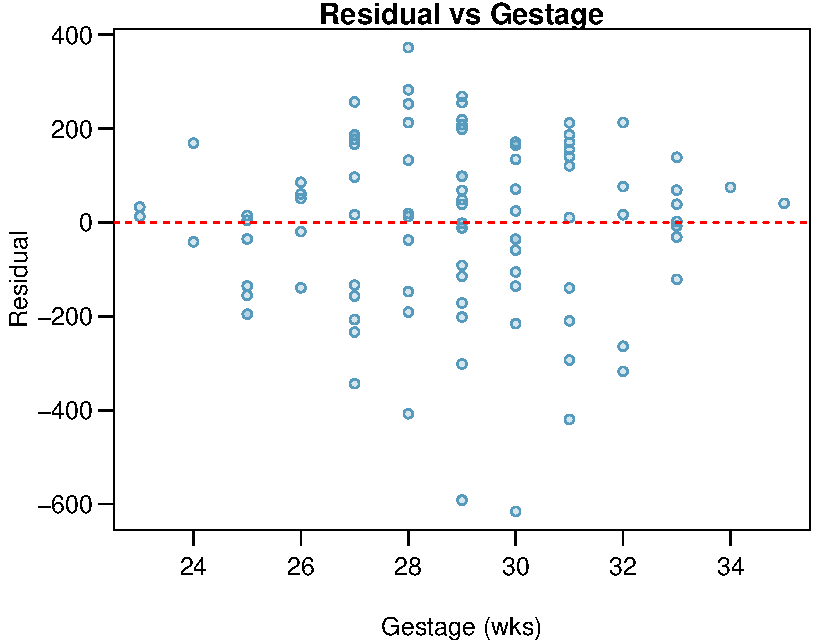
\includegraphics[width=0.32\textwidth]{ch_multiple_linear_regression_oi_biostat/figures/eoce/bwt_toxemia/low_bwt_pred.pdf}
	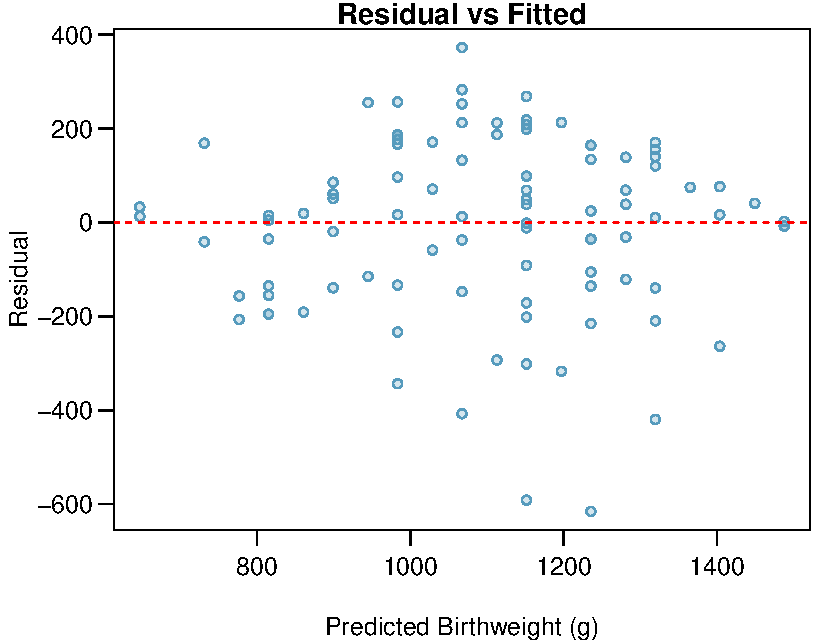
\includegraphics[width=0.32\textwidth]{ch_multiple_linear_regression_oi_biostat/figures/eoce/bwt_toxemia/low_bwt_predicted.pdf}
	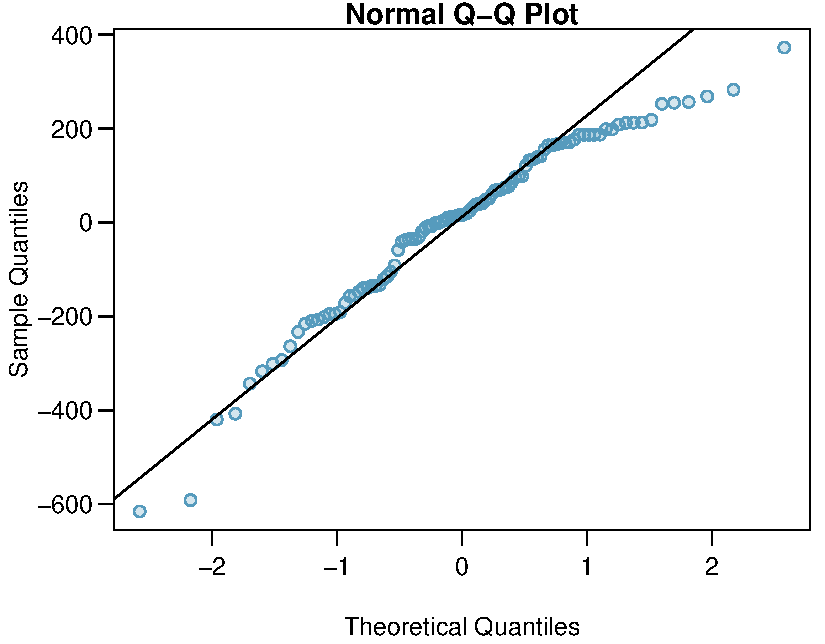
\includegraphics[width=0.32\textwidth]{ch_multiple_linear_regression_oi_biostat/figures/eoce/bwt_toxemia/low_bwt_qq.pdf}
\end{center}

\begin{parts}
	\item Write the model equation.
	
	\item Interpret the coefficients of the model, and comment on whether the intercept has a meaningful interpretation.
	
	\item Predict the average birth weight for an infant born to a mother diagnosed with toxemia with gestational age 31 weeks.
	
	\item Evaluate whether the assumptions for linear regression are reasonably satisfied.
	
	\item A simple regression model with only toxemia status as a predictor had $R^2 = 0.0001$ and $R^2_{adj} = 0.010$; in this model, the slope estimate for toxemia status is 7.785, with $p = 0.907$. The simple regression model and multiple regression model disagree regarding the nature of the association between birth weight and toxemia. Briefly explain a potential reason behind the discrepancy. Which model do you prefer for understanding the relationship between birth weight and toxemia, and why?
\end{parts}
}{}

% 9 ODD (OI4, 9.19) edited

\eoce{\qt{Multiple regression fact checking\label{mult_regr_facts}}
Determine which of the following statements are
true and false.
For each statement that is false, explain why it is false.
\begin{parts}
%\item
    %If predictors are collinear, then removing
    %one variable will have no influence on the
    %point estimate of another variable's coefficient.
\item
    Suppose a numerical variable $x$ has a coefficient of
    $b_1 = 2.5$ in the multiple regression model.
    Suppose also that the first observation has $x_1 = 7.2$,
    the second observation has a value of $x_1 = 8.2$,
    and these two observations have the same values
    for all other predictors.
    Then the predicted value of the second observation
    will be 2.5 higher than the prediction of the first
    observation based on the multiple regression model.
\item
    If a regression model's first variable has
    a coefficient of $b_1 = 5.7$, then if we are
    able to influence the data so that an observation
    will have its $x_1$ be 1 larger than it would
    otherwise, the value $y_1$ for this observation
    would increase by 5.7.
\item
    Suppose we fit a multiple regression model
    based on a data set of 472 observations.
    We also notice that the distribution of the
    residuals includes some skew but does not
    include any particularly extreme outliers.
    Because the residuals are not nearly normal,
    we should not use this model and require
    more advanced methods to model these data.
\end{parts}
}{}


\textD{\newpage}


\subsection{The general multiple regression model}

% 10 (OI4, 9.6)

\eoce{\qt{Cherry trees\label{cherry_trees}} Timber yield is approximately equal to the 
	volume of a tree, however, this value is difficult to measure without first 
	cutting the tree down. Instead, other variables, such as height and diameter, 
	may be used to predict a tree's volume and yield. Researchers wanting to 
	understand the relationship between these variables for black cherry trees 
	collected data from 31 such trees in the Allegheny National Forest, 
	Pennsylvania. Height is measured in feet, diameter in inches (at 54 inches above 
	ground), and volume in cubic feet.\footfullcite{Hand:1994}

		\begin{center}
			\begin{tabular}{rrrrr}
				\hline
				& Estimate  & Std. Error  & t value   & Pr($>$$|$t$|$) \\ 
				\hline
				(Intercept) & -57.99    & 8.64        & -6.71     & 0.00 \\ 
				height      & 0.34      & 0.13        & 2.61      & 0.01 \\ 
				diameter    & 4.71      & 0.26        & 17.82     & 0.00 \\ 
				\hline
			\end{tabular}
		\end{center}

	\begin{parts}
		\item Calculate a 95\% confidence interval for the coefficient of height, and 
		interpret it in the context of the data.
		\item One tree in this sample is 79 feet tall, has a diameter of 11.3 inches, 
		and is 24.2 cubic feet in volume. Determine if the model overestimates or 
		underestimates the volume of this tree, and by how much.
	\end{parts}
}{}

% 11 (OI4, 9.5)

\eoce{\qt{GPA\label{gpa}} A survey of 55 Duke University students asked about their 
	GPA, number of hours they study at night, number of nights they go out, and 
	their gender. Summary output of the regression model is shown below. Note that 
	male is coded as 1. 
	\begin{center}
		\begin{tabular}{rrrrr}
			\hline
			& Estimate  & Std. Error  & t value   & Pr($>$$|$t$|$) \\ 
			\hline
			(Intercept) & 3.45      & 0.35        & 9.85      & 0.00 \\ 
			studyweek   & 0.00      & 0.00        & 0.27      & 0.79 \\ 
			sleepnight  & 0.01      & 0.05        & 0.11      & 0.91 \\ 
			outnight    & 0.05      & 0.05        & 1.01      & 0.32 \\ 
			gender      & -0.08     & 0.12        & -0.68     & 0.50 \\ 
			\hline
		\end{tabular}
	\end{center}
	\begin{parts}
		\item Calculate a 95\% confidence interval for the coefficient of gender in the 
		model, and interpret it in the context of the data.
		\item Would you expect a 95\% confidence interval for the slope of the remaining 
		variables to include 0? Explain
	\end{parts}
}{}

% 12 oi_biostat

\eoce{\qt{Trait inheritance of high blood pressure\label{inherit_bp}} One research question of public health interest is to determine the extent to which high blood pressure is a genetic phenomenon.  In 20 families, the systolic blood pressure of the mother, father, and first-born child in the family were measured (in units of mm Hg).  A multiple linear regression model using $Y$ = child’s blood pressure, $X_1$ = mother’s blood pressure, and $X_2$ = father’s blood pressure led to the following estimate of a least squares line: $E(Y) = -15.69 + 0.415X_1 + 0.423X_2$. The standard errors associated with $b_0$, $b_1$, and $b_2$, respectively, are 23.65, 0.125, and 0.119. The least squares fit produced $R^2 = 0.597$ and $MSE =  113.8$. 

\begin{parts}
	
	\item What proportion of the variability of a child's systolic blood pressure is explained by this model?
	
	\item Does the least squares line indicate statistically significant associations between each of the parent's systolic blood pressures and that of the child? Explain your answer.
	
	\item What is the predicted systolic blood pressure for a child whose mother's and father's systolic blood pressure is 125 mm Hg and 140 mm Hg, respectively?
	
	%\item Calculate an approximate 95\% confidence interval for this predicted value. 
	
	\item A colleague tells you that something must be wrong with your model because your fitted intercept is negative, but blood pressures are never negative.  How do you respond?
	
	\item Briefly describe three different plots for assessing the appropriateness or fit of the above regression model.
	
\end{parts}

}{}

\textD{\newpage}

% 13 oi_biostat

\eoce{\qt{Wolbachia, Part II\label{wolbachia_inf}} Exercise~\ref{wolbachia_intro} introduced a study about Wolbachia and reproductive success in a wasp host. The following table shows the model coefficients for a model predicting the number of eggs laid over a lifetime from the predictor variables wolbachia density and tibia length. A higher number of eggs laid over a lifetime is indicative of greater reproductive success. The model has $R^2 = 0.314$ and degrees of freedom 34. The $F$-statistic is 7.782, with $p$-value 0.0016.
	
	\begin{center}
	\begin{tabular}{rrrrr}
		\hline
		& Estimate  & Std. Error  & t value   & Pr($>$$|$t$|$) \\ 
		\hline
		(Intercept) & -17.88    & 28.63      & -0.62  & 0.537 \\ 
		wolbachia       & 4.28   & 1.25    & 3.42  & 0.002 \\ 
		tibia & 0.272 & 0.16 & 1.69 & 0.010 \\
		\hline
	\end{tabular}
	\end{center}	

\begin{parts}
	\item Write the model equation.
	\item Interpret the slope coefficient of \texttt{wolbachia}.
	\item Assess the evidence for whether \textit{Wolbachia} is beneficial for its host in nature, based on these data.
	\item Compute and interpret a 95\% confidence interval for the population slope of \texttt{wolbachia}.
	\item Interpret the significance of the $F$-statistic.
\end{parts}


}{}

% 14 oi_biostat pset 7, spring 2020

\eoce{\qt{Difficult encounters, Part I\label{ddprq_intro}} A study was conducted at a university outpatient primary care clinic in Switzerland to identify factors associated with difficult doctor-patient encounters. The data consist of 527 patient encounters, conducted by the 27 medical residents employed at the clinic. After each encounter, the attending physician completed two questionnaires: the Difficult Doctor Patient Relationship Questionnaire (DDPRQ-10) and the patient's vulnerability grid (PVG).
	
	A higher score on the DDPRQ-10 indicates a more difficult encounter. The maximum possible score is 60 and encounters with score 30 and higher are considered difficult.
	
	A model was fit for the association of DDPRQ-10 score with features of the attending physician: age, sex, and years of training. The model has $F$-statistic of 0.23 on 3 and 286 degrees of freedom, with $p$-value 0.876.
	
	\begin{center}
		\begin{tabular}{rrrrr}
			\hline
			& Estimate  & Std. Error  & t value   & Pr($>$$|$t$|$) \\ 
			\hline
			(Intercept) & 30.594   & 2.886      & 10.601 & 0.0000 \\ 
			age      & -0.016  & 0.104    & -0.157 & 0.876 \\ 
			sexM & -0.535 & 0.781 & -0.686 & 0.494 \\
			yrs.train & 0.096 & 0.215 & 0.445 & 0.656 \\
			\hline
		\end{tabular}
	\end{center}	

	\begin{parts}
		\item As a group, are these physician features useful for predicting DDPRQ-10 score?
		
		\item Is there evidence of a significant association between DDPRQ-10 score and any of the physician features?
	\end{parts}
}


\textD{\newpage}


\subsection{Categorical predictors with more than two levels}

% 15 oi_biostat

\eoce{\qt{Prison isolation experiment, Part III\label{prison_isolation_regression}}

Exercises~\ref{prison_isolation_T} and \ref{prison_isolation_anova} introduced an experiment conducted with the goal of identifying a treatment that reduces subjects' psychopathic deviant T scores on the MMPI test.  Exercise~\ref{prison_isolation_T} evaluated the success of each individual treatment, and in exercise~\ref{prison_isolation_anova}, ANOVA was used to compare the success of the three treatments. This exercise uses multiple regression to examine the intervention effect.

For this problem, a treatment variable (labeled \texttt{treatment}) has been constructed with three levels:

\begin{enumerate}[(1)]
	\setlength{\itemsep}{0mm}
	\item \texttt{Therapeutic} for sensory restriction plus the 15 minute "therapeutic" tape advising that professional help is available.
	\item \texttt{Neutral} for sensory restriction plus a 15 minute "emotionally neutral" tap on training hunting dogs.
	\item \texttt{Absent} for sensory restriction but no taped message. 
\end{enumerate}

Forty-two subjects were randomly assigned to these treatment groups, and an MMPI test was administered before and after the treatment. Investigators hoped that the interventions would lower MMPI scores. The table below shows the result of a multiple regression in \textsf{R} where the response variable \texttt{trt.effect} is the change in MMPI score (pre-intervention - post-intervention) and the predictor variable is \texttt{treatment}.

% latex table generated in R 3.6.2 by xtable 1.8-4 package
% Thu May 21 11:13:47 2020
	\begin{center}
	\begin{tabular}{rrrrr}
		\hline
		& Estimate & Std. Error & t value & Pr($>$$|$t$|$) \\ 
		\hline
		(Intercept) & -3.2143 & 2.6174 & -1.23 & 0.2268 \\ 
		treatmentNeutral & 6.0714 & 3.7015 & 1.64 & 0.1090 \\ 
		treatmentTherapeutic & 9.4286 & 3.7015 & 2.55 & 0.0149 \\ 
		\hline
	\end{tabular}
	\end{center}

In this model, the residual standard error is 9.79, the $F$-statistic is 3.33 with 2 and 39 degrees of freedom; $P(F_{2,39} > 3.33) = 0.0461$.

\begin{parts}
	
	\item Interpret the meaning of a positive value for \texttt{trt.effect} versus a negative value.
	
	\item Write the estimated model equation.
	
	\item Calculate the predicted value for \texttt{trt.effect} for a patient in the neutral tape group. 
	
	\item Does the intercept have a meaningful interpretation in this model?
	
	\item What is the interpretation of the two slope coefficients in the regression model?
	
	\item Describe the tested hypotheses that correspond to each of the $p$-values in the last column of the table.
	
\end{parts}	

}{}

% 16 oi_biostat pset 7, spring 2020

\eoce{\qt{Poverty and educational level\label{nhanes_poverty}} This question uses data from 500 randomly selected adults in the larger NHANES dataset. \texttt{Poverty} is measured as a ratio of family income to poverty guidelines. Smaller numbers indicate more poverty, and ratios of 5 or larger were recorded as 5. The \texttt{Education} variable indicates the highest level of education achieved: either 8th grade, 9 - 11th grade, high school, some college, or college grad.

% latex table generated in R 3.6.2 by xtable 1.8-4 package
% Thu Jun 04 17:10:39 2020
	\begin{center}
	\begin{tabular}{rrrrr}
		\hline
		& Estimate & Std. Error & t value & Pr($>$$|$t$|$) \\ 
		\hline
		(Intercept) & 1.4555 & 0.2703 & 5.38 & 0.0000 \\ 
		Education9 - 11th Grade & 0.9931 & 0.3302 & 3.01 & 0.0028 \\ 
		EducationHigh School & 1.0900 & 0.3113 & 3.50 & 0.0005 \\ 
		EducationSome College & 1.4943 & 0.2976 & 5.02 & 0.0000 \\ 
		EducationCollege Grad & 2.4948 & 0.2958 & 8.43 & 0.0000 \\ 
		\hline
	\end{tabular}
	\end{center}

In this model, the residual standard error is 1.46, the $F$-statistic is 28.09 with 4 and 456 degrees of freedom; $P(F_{4, 456} > 28.09) < 0.0001$.

\begin{parts}
	
	\item Write the estimated model equation.
	
	\item Calculate the predicted poverty ratio for an individual who at most completed high school.
	
	\item Interpret the estimated intercept value.
	
	\item Interpret the slope coefficient for \texttt{EducationCollege Grad}, and describe the tested hypotheses that correspond to the $p$-value for this slope coefficient.
	
	\item Assess whether educational level, overall, is associated with poverty. Be sure to include any relevant numerical evidence as part of your answer.
	
\end{parts}


}{}

% 17 oi_biostat

\eoce{\qt{Prison isolation experiment, Part IV\label{prison_isolation_general}} Exercise~\ref{prison_isolation_regression} used regression to examine the effect of three interventions on prisoner MMPI scores.  The response variable in the regression was \texttt{trt.effect}, the change in MMPI score (pre-intervention - post-intervention). 

Instead of estimating the intervention effect through the change in scores, suppose one is interested in predicting a post-intervention score based on the pre-intervention score for an individual and a particular intervention. 

\begin{parts}
	
	\item The table below shows an alternative regression model that can be fit to the data.  In this model, the response variable is the post-intervention MMPI value (\texttt{post}, not shown explicitly in the table) and the predictors are the pre-intervention score (\texttt{pre}) and the treatment, coded as in problem~\ref{prison_isolation_regression}. 
	
	Write the estimated equation for this model.
	
	% latex table generated in R 3.6.2 by xtable 1.8-4 package
	% Thu May 21 18:32:36 2020
		\begin{center}
		\begin{tabular}{rrrrr}
			\hline
			& Estimate & Std. Error & t value & Pr($>$$|$t$|$) \\ 
			\hline
			(Intercept) & 28.4053 & 12.2949 & 2.31 & 0.0264 \\ 
			pre & 0.6593 & 0.1628 & 4.05 & 0.0002 \\ 
			treatmentNeutral & -5.7307 & 3.5545 & -1.61 & 0.1152 \\ 
			treatmentTherapeutic & -9.7450 & 3.5540 & -2.74 & 0.0093 \\ 
			\hline
		\end{tabular}
		\end{center}
	
	\item In this model, describe in general terms the association of the pre-intervention and post-intervention scores.
	
	\item Does the pre-intervention score appear to be an important predictor of a post intervention score?
	
	\item What is the  predicted post-intervention score for an individual with a pre-intervention score of 73 and receiving no tape after the isolation?
	
	\item Explain the interpretation of the coefficients for coefficient of \texttt{treatmentNeutral}.  Is there strong statistical evidence that it is an important predictor?

\end{parts}

}{}	
	
	
% 18 oi_biostat

\eoce{\qt{Resilience, Part I\label{resilience_cat}} The American Psychological Association defines resilience as "the process of adapting well in the face of adversity, trauma, tragedy, threats, or even significant sources of stress". Studies have suggested that resilience is an important factor in contributing to how medical students perceive their quality of life and educational environment.
	
	Survey data were collected from 1,350 students across 25 medical schools. At each school, 54 students were randomly selected to participate in the study. Participants completed questionnaires measuring resilience, quality of life, perception of educational environment, depression symptoms, and anxiety symptoms.
	
	The following regression model was fit to analyze the relationship between resilience and depressive symptoms. Resilience was categorized as: very low, low, moderately low, moderately high, high, and very high. Depressive symptoms were measured on a scale of 0 to 63 points, with higher scores indicating either more numerous or more severe depressive symptoms; this questionnaire is called the Beck Depression Inventory (BDI).
	
	In this model, the residual standard error is 5.867, the $F$-statistic is 118.1 with 5 and 1344 degrees of freedom; $P(F_{5, 1344} > 118.1) < 0.0001$.
	
	% latex table generated in R 3.6.2 by xtable 1.8-4 package
	% Thu Jun 04 19:50:47 2020
	\begin{center}
		\begin{tabular}{rrrrr}
			\hline
			& Estimate & Std. Error & t value & Pr($>$$|$t$|$) \\ 
			\hline
			(Intercept) & 4.9754 & 0.4118 & 12.08 & 0.0000 \\ 
			resHigh & 2.2936 & 0.4987 & 4.60 & 0.0000 \\ 
			resModHigh & 4.3005 & 0.5181 & 8.30 & 0.0000 \\ 
			resModLow & 6.7108 & 0.5938 & 11.30 & 0.0000 \\ 
			resLow & 9.6538 & 0.7458 & 12.94 & 0.0000 \\ 
			resVeryLow & 15.6453 & 0.7518 & 20.81 & 0.0000 \\ 
			\hline
		\end{tabular}
	\end{center}

	\begin{parts}
		
		\item Describe the overall trend in language accessible to someone who has not taken a statistics course. 
		
		\item Does the intercept have a meaningful interpretation? Explain your answer.
		
		\item Compare the predicted mean BDI score for someone with low resilience to that of someone with very low resilience.

		\item[(d) + (e)] \textbf{Continue to the next page for parts (d) and (e).}
		
\textD{\newpage}

		\item Assess whether level of resilience, overall, is associated with depressive symptoms as measured by BDI score. Be sure to include any relevant numerical evidence as part of your answer.
		
		\item A model was fitted predicting BDI score from resilience, with the categories numerically coded from \texttt{1} to \texttt{6}, with \texttt{1} being very high resilience and \texttt{6} being very low resilience. This model has a single slope estimate of 2.76 with $p$-value < 0.0001. 
		
		\begin{subparts}
			\item Using this model, compare the predicted mean BDI score for someone with low resilience to that of someone with very low resilience. Compare this answer to the one from part (c).
			
			\item What does this model imply about the change in mean BDI score between groups?
			
			\item Explain why this model is flawed.
			
		\end{subparts}
	\end{parts}
}{}

\subsection{Interaction in regression}

% 19 oi_biostat

\eoce{\qt{Prison isolation experiment, Part V\label{prison_isolation_interaction}} Exercise~\ref{prison_isolation_general} used regression to predict a post-intervention score based on pre-intervention score and a particular intervention.
	
	The following table shows a model incorporating interaction between pre-intervention score and intervention.
	
	% latex table generated in R 3.6.2 by xtable 1.8-4 package
	% Fri Jun 05 16:03:17 2020
	\begin{center}
		\begin{tabular}{rrrrr}
			\hline
			& Estimate & Std. Error & t value & Pr($>$$|$t$|$) \\ 
			\hline
			(Intercept) & -17.5790 & 17.7090 & -0.99 & 0.3275 \\ 
			pre & 1.2813 & 0.2376 & 5.39 & 0.0000 \\ 
			treatmentNeutral & 67.7518 & 30.6168 & 2.21 & 0.0333 \\ 
			treatmentTherapeutic & 64.4183 & 24.2124 & 2.66 & 0.0116 \\ 
			pre:treatmentNeutral & -0.9890 & 0.4082 & -2.42 & 0.0206 \\ 
			pre:treatmentTherapeutic & -1.0080 & 0.3266 & -3.09 & 0.0039 \\ 
			\hline
		\end{tabular}
	\end{center}
	
	\begin{parts}
		
		\item Write the model equation.
		
		\item Interpret the model coefficients.
		
		\item Write a separate model equation for each intervention group.
		
		\item Do these data suggest that there is a statistically significant difference in association between pre- and post-intervention scores by treatment group? Explain your answer.
		
	\end{parts}
	
}{}

% 20 oi_biostat pset 7, spring 2020

\eoce{\qt{Vitamin D\label{thai_vitamin_d}} A study was conducted to evaluate Vitamin D status among schoolchildren in Thailand. Exposure to sunlight allows the body to produce serum $25(OH)D$, which is a marker of Vitamin D status; serum level is measured in units of nmol/L and having serum level below 50 nmol/L is indicative of Vitamin D deficiency. The following model was fit to predict serum $25(OH)D$ level from age, sex, and their interaction.
	
	% latex table generated in R 3.6.2 by xtable 1.8-4 package
	% Fri Jun 05 16:15:51 2020
	\begin{center}
		\begin{tabular}{rrrrr}
			\hline
			& Estimate & Std. Error & t value & Pr($>$$|$t$|$) \\ 
			\hline
			(Intercept) & 97.7709 & 4.7732 & 20.48 & 0.0000 \\ 
			age & -3.0156 & 0.4774 & -6.32 & 0.0000 \\ 
			sexM & -16.2848 & 7.0740 & -2.30 & 0.0217 \\ 
			age:sexM & 2.9369 & 0.7054 & 4.16 & 0.0000 \\ 
			\hline
		\end{tabular}
	\end{center}
	
	\begin{parts}
		
		\item Write the model equation.
		
		\item Interpret the model coefficients.
		
		\item Is there statistically significant evidence that the association between serum $25(OH)D$ level and age differs by sex? Explain your answer.
		
	\end{parts}
	
}{}

\textD{\newpage}

% 21 oi_biostat

\eoce{\qt{PREVEND, Part III\label{prevend_interact}} Exercise~\ref{prevend_interpret} showed a multiple regression model predicting RFFT score from statin use and age. For this problem, an interaction term is added between statin use and age.
	
	% latex table generated in R 3.6.2 by xtable 1.8-4 package
	% Fri Jun 05 16:24:12 2020
	\begin{center}
		\begin{tabular}{rrrrr}
			\hline
			& Estimate & Std. Error & t value & Pr($>$$|$t$|$) \\ 
			\hline
			(Intercept) & 140.2031 & 5.6209 & 24.94 & 0.0000 \\ 
			Statin & -13.9720 & 15.0113 & -0.93 & 0.3524 \\ 
			Age & -1.3149 & 0.1040 & -12.65 & 0.0000 \\ 
			Statin:Age & 0.2474 & 0.2468 & 1.00 & 0.3166 \\ 
			\hline
		\end{tabular}
	\end{center}

	\begin{parts}
		
		\item Write the model equation.
		
		\item Interpret the model coefficients.
		
		\item Is there statistically significant evidence that the association between RFFT score and age differs by whether someone is a statin user? Explain your answer.
		
	\end{parts}
}{}


% 22 oi_biostat spring 2020 final exam

\eoce{\qt{Antibiotic consumption, Part I\label{antibiotic_interact}} Antibiotic resistance represents a major public health challenge. Overuse of antibiotics in clinical settings is thought to be a major contributor to increased antibiotic resistance. A study was conducted across several regions in China to investigate the impact of a 2011 law prohibiting over-the-counter (OTC) sales of antibiotics in private pharmacies. The study team collected data on average monthly antibiotic consumption in 621 counties, in addition to information on socioeconomic determinants such as percentage of population illiterate.
	
	The following model was fit to investigate whether the relationship between monthly antibiotic consumption and percentage of population (over 25 years of age) with an advanced degree differs between counties that are located in a metropolitan area and those that are not.
	
	% latex table generated in R 3.6.2 by xtable 1.8-4 package
	% Fri Jun 05 16:40:07 2020
	\begin{center}
		\begin{tabular}{rrrrr}
			\hline
			& Estimate & Std. Error & t value & Pr($>$$|$t$|$) \\ 
			\hline
			(Intercept) & 0.8482 & 0.3311 & 2.56 & 0.0107 \\ 
			metroYes & 2.3035 & 0.9612 & 2.40 & 0.0169 \\ 
			edu & 0.5711 & 0.0319 & 17.90 & 0.0000 \\ 
			metroYes:edu & -0.1838 & 0.0752 & -2.44 & 0.0148 \\ 
			\hline
		\end{tabular}
	\end{center}

	\begin{parts}
		\item Interpret the model coefficients, including any relevant inferential results.
		
		\item Make a prediction of average monthly antibiotic consumption for a county in a metropolitan area where 10\% of the population over 25 years old has an advanced degree.
		
	\end{parts}

}


\subsection{Model selection for explanatory variables}

% 23 ODD (OI4, 9.7) edited

\eoce{\qt{Baby weights, Part VII\label{baby_weights_remove}} Suppose the starting point for model selection for the birth weight data were the full model, with all variables. The table below shows the adjusted $R^2$ for the full model as well as the adjusted $R^2$ values for all models with one fewer predictor variable. Based on examining the table from Exercise~\ref{baby_weights_mlr} and the following table, identify which variable, if any, should be removed from the model first. Explain your answer.

\begin{center}
	\begin{tabular}{rlr}
		\hline
		& Model               & Adjusted $R^2$ \\ 
		\hline
		1 & Full model          & 0.2541 \\ 
		2 & No gestation        & 0.1031 \\ 
		3 & No parity           & 0.2492 \\ 
		4 & No age              & 0.2547 \\ 
		5 & No height           & 0.2311 \\ 
		6 & No weight           & 0.2536 \\ 
		7 & No smoking status   & 0.2072 \\ 
		\hline
	\end{tabular}
\end{center}
}

\textD{\newpage}

% 24 EVEN (OI4, 9.8) edited

\eoce{\qt{Absenteeism, Part II\label{absent_from_school_remove}} Suppose the starting point for model selection for the absenteeism data were the full model, with all variables. The table below shows the adjusted $R^2$ for the full model as well as the adjusted $R^2$ values for all models with one fewer predictor variable. Based on examining the table from Exercise~\ref{absent_from_school_mlr} and the following table, identify which variable, if any, should be removed from the model first. Explain your answer.

\begin{center}
	\begin{tabular}{rlr}
		\hline
		& Model               & Adjusted $R^2$ \\ 
		\hline
		1 & Full model          & 0.0701 \\ 
		2 & No ethnicity        & -0.0033 \\ 
		3 & No sex              & 0.0676 \\ 
		4 & No learner status   & 0.0723 \\ 
		\hline
	\end{tabular}
\end{center}
	
}{}

% 25 oi_biostat

\eoce{\qt{Baby weights, Part VIII\label{baby_weights_exploratory}} Exercise~\ref{baby_weights_mlr} shows a regression model for predicting the average birth weight of babies based on all variables included in the dataset: length of pregnancy in days (\texttt{gestation}), mother's age in years (\texttt{age}), mother's height in inches (\texttt{height}), and mother's pregnancy weight in pounds (\texttt{weight}).
	
	The following plots show the relationships between the response and the numerical predictor variables, in addition to the relationships between the response and two categorical predictor variables.
	
	\begin{center}	
		\includegraphics[width=0.7\textwidth]{ch_multiple_linear_regression_oi_biostat/figures/eoce/baby_weights_matrix/babiesBoxPlots.pdf}
	\end{center}
	
	\begin{center}
		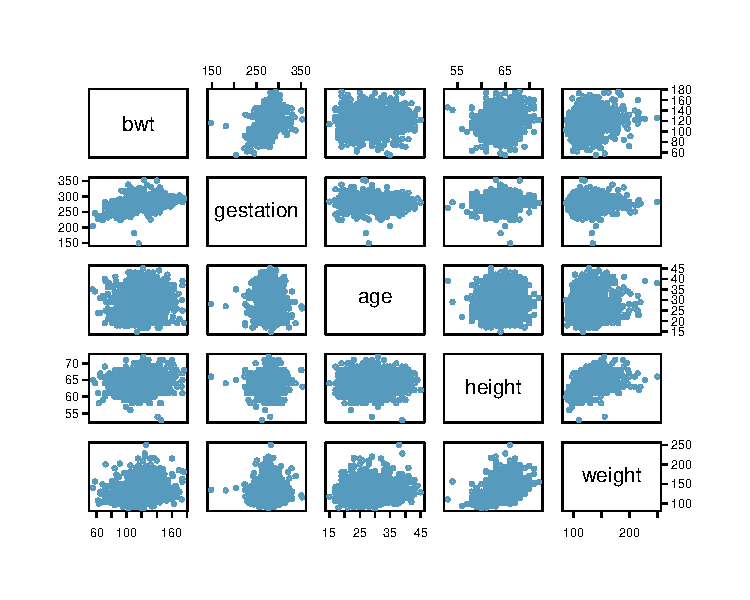
\includegraphics[width=0.8\textwidth]{ch_multiple_linear_regression_oi_biostat/figures/eoce/baby_weights_matrix/babiesScatterPlotMatrix.pdf}		
	\end{center}
	
	\begin{parts}
		
		\item Examine the relationship between the response variable and the predictor variables. Describe what you see. Which predictor variables seem like they would be useful to include in an initial model?
		
		\item Identify any predictors that seem related to each other.
		
	\end{parts}
	
}{}

\textD{\newpage}

% 26 oi_biostat

\eoce{\qt{Antibiotic consumption, Part II\label{antibiotic_consumption_select}} Exercise~\ref{antibiotic_interact} introduced a study conducted about antibiotic consumption in China. One aim of the study was to develop a prediction model for predicting monthly average antibiotic consumption based on county-level data. The following plots show the association between monthly average antibiotic consumption and four potential predictor variables: proportion female inhabitants (\texttt{female}), average life expectancy in years (\texttt{lifeexp}), proportion of population illiterate (\texttt{illiterate}), and population density in 1,000 people / $km^2$ (\texttt{popdensity}).
	
	\begin{center}
		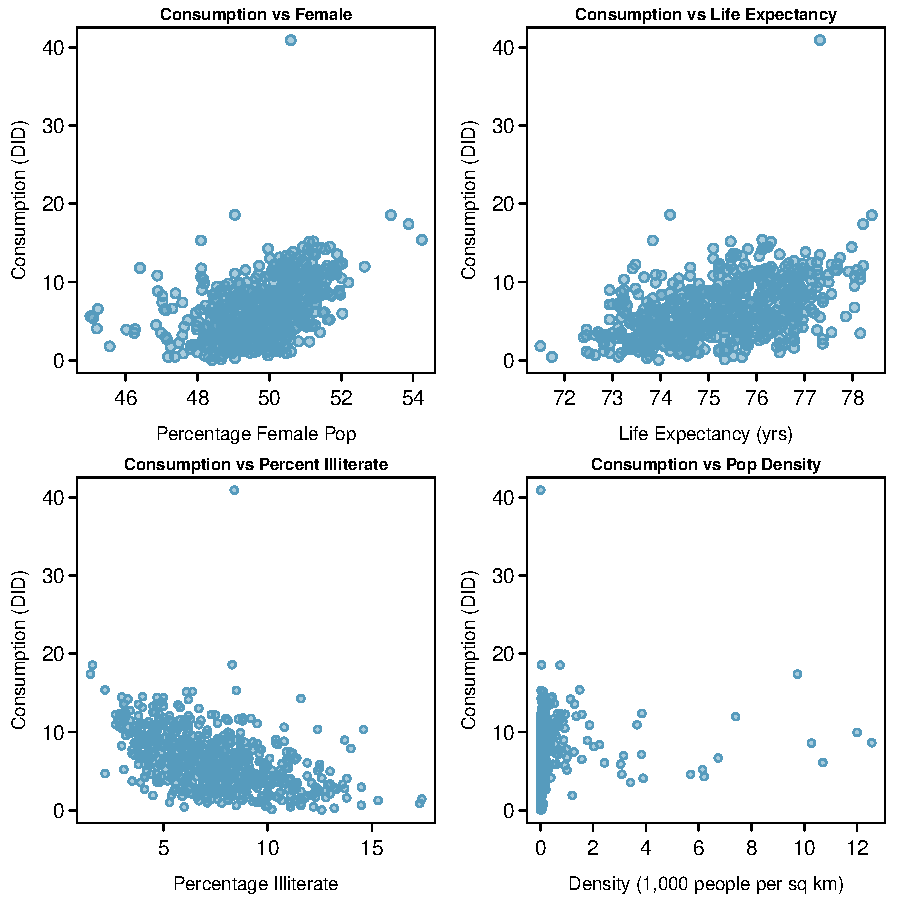
\includegraphics[width=0.9\textwidth]{ch_multiple_linear_regression_oi_biostat/figures/eoce/antibiotic/antibioticsPlots.pdf}		
	\end{center}
	
	\begin{parts}
		\item Summarize what you see.
		
		\item Identify any predictor variables that might benefit from a natural log transformation and briefly justify your choices.
	\end{parts}

}{}


\textD{\newpage}


\subsection{The connection between ANOVA and regression}

% 27 oi_biostat

\eoce{\qt{Prison isolation experiment, Part VI\label{prison_isolation_anova_reg}} Problem~\ref{prison_isolation_regression} used a regression model to examine the effect of the interventions on possibly reducing psychopathic deviant T scores on prisoners.  The regression model is shown in the problem statement. 

\begin{parts}
	
	\item The value of the $F$-statistic is 3.33 with 2 and 39 degrees of freedom and $P(F_{2,39} > 3.33) = 0.0461$. In terms of the variables in the regression model, state the null hypothesis that corresponds to the $F$-statistic.
	
	\item Describe the relationship between the coefficients from the linear model and the usual summary statistics for the three sets of difference scores.
	
	\item Explain why the null hypothesis in this regression model is equivalent to the null hypothesis when these data were analyzed using ANOVA in Problem~\ref{prison_isolation_anova}.
	
	\item Explain whether the assumptions for this regression model differ from those used in ANOVA.
	
\end{parts}

}{}

% 28 oi_biostat

\eoce{\qt{Resilience, Part II\label{resilience_anova_reg}} Exercise~\ref{resilience_cat} shows a regression model for the association of BDI score with resilience level. 
	
	\begin{parts}
		
		\item In terms of the variables in the regression model, state the null hypothesis that corresponds to the $F$-statistic.
		
		\item Describe the relationship between the coefficients from the linear model and the usual summary statistics for the six sets of BDI scores.
		
		\item Explain why the null hypothesis used in this regression model is equivalent to the null hypothesis that would be used if these data were analyzed with an ANOVA approach.
		
		%\item Comment on the difference between what an ANOVA summary output would provide for these data versus what is shown in Exercise~\ref{resilience_cat}.
		
	\end{parts}

}{}